\documentclass{beamer}
\usepackage{progressbar, tcolorbox, CJKutf8, hyperref, multicol, pdfpages, graphicx, xcolor, blindtext, tikz, smartdiagram, listings}
\usepackage[absolute,overlay]{textpos}
\usepackage[backend=bibtex,style=numeric,sorting=none]{biblatex}

\hypersetup{
    colorlinks=true,
    linkcolor=blue,
    filecolor=magenta,      
    urlcolor=blue,
    }

    \definecolor{mygreen}{rgb}{0,0.6,0}
    \definecolor{mygray}{rgb}{0.5,0.5,0.5}
    \definecolor{mymauve}{rgb}{0.58,0,0.82}


    \lstset{ 
      backgroundcolor=\color{white},   % choose the background color; you must add \usepackage{color} or \usepackage{xcolor}; should come as last argument
      basicstyle=\ttfamily\footnotesize,% the size of the fonts that are used for the code
      breakatwhitespace=false,         % sets if automatic breaks should only happen at whitespace
      breaklines=true,                 % sets automatic line breaking
      captionpos=b,                    % sets the caption-position to bottom
      commentstyle=\color{mygreen},    % comment style
      deletekeywords={...},            % if you want to delete keywords from the given language
      escapeinside={\%*}{*)},          % if you want to add LaTeX within your code
      extendedchars=true,              % lets you use non-ASCII characters; for 8-bits encodings only, does not work with UTF-8
      frame=single,	                   % adds a frame around the code
      keepspaces=true,                 % keeps spaces in text, useful for keeping indentation of code (possibly needs columns=flexible)
      keywordstyle=\color{magenta},        % keyword style
      morekeywords={FROM, RUN, ENV, USER, WORKDIR, CMD, EXPOSE, ADD, COPY, sudo, curl, chmod, ln, git, cd},
                                       % if you want to add more keywords to the set
      numbers=left,                    % where to put the line-numbers; possible values are (none, left, right)
      numbersep=5pt,                   % how far the line-numbers are from the code
      numberstyle=\tiny\color{mygray}, % the style that is used for the line-numbers
      rulecolor=\color{black},         % if not set, the frame-color may be changed on line-breaks within not-black text (e.g. comments (green here))
      showspaces=false,                % show spaces everywhere adding particular underscores; it overrides 'showstringspaces'
      showstringspaces=false,          % underline spaces within strings only
      showtabs=false,                  % show tabs within strings adding particular underscores
      stepnumber=1,                    % the step between two line-numbers. If it's 1, each line will be numbered
      stringstyle=\color{mymauve},     % string literal style
      tabsize=4,	                     % sets default tabsize to ˋ spaces
      title=\lstname
    }

\graphicspath{ {./images/} }
\usetheme{AnnArbor}
\addbibresource{main.bib}
\usetikzlibrary{positioning, calc, shapes.multipart, shapes.arrows, fit, backgrounds}

\definecolor{dockerColor}{RGB}{13, 183, 237}
\definecolor{secureColor}{RGB}{10, 191, 83}
\definecolor{aquamarine}{rgb}{0.5, 1.0, 0.83}
\definecolor{aquamarine2}{rgb}{0.2, 1.0, 0.53}

\title{The Container Security in Healthcare Data Exchange System}
\subtitle{Bachelor's degree graduation project}
\author{Chih-Hsuan Yang}
\institute{National Sun Yat-sen University\\
Advisor: Chun-I Fan
}
\date{\today}

\AtBeginSection[]{
  \begin{frame}
  \vfill
  \centering
  \begin{beamercolorbox}[sep=8pt,center,shadow=true,rounded=true]{title}
    \usebeamerfont{title}\insertsectionhead\par%
  \end{beamercolorbox}
  \vfill
  \end{frame}
}

\def\checkmark{\tikz\fill[scale=0.4](0,.35) -- (.25,0) -- (1,.7) -- (.25,.15) -- cycle;} 

\begin{document}
\begin{CJK*}{UTF8}{bsmi}

  \begin{frame}
    \titlepage
  \end{frame}


  \begin{frame}{Outline}
    \begin{multicols}{2}
      \tableofcontents
    \end{multicols}
  \end{frame}

  \begin{frame}{Flow chart}
    \centering
    \scalebox{0.9} {
      \smartdiagram[flow diagram:horizontal]{
        Scan base, Sign, Image checking, Start policy, Runtime enforcement
      }
    }
  \end{frame}

  \section{Soul}
  \begin{frame}{Malicious behavior}
    \centering
    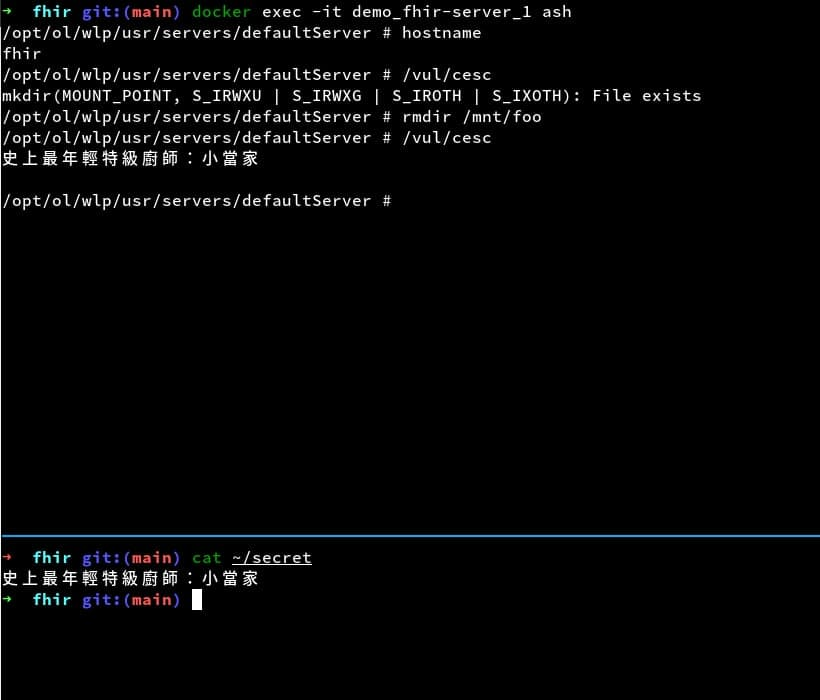
\includegraphics[height=\textheight]{photo_2021-09-17_05-53-42.jpg}
  \end{frame}

  \begin{frame}{My soultion}
    Block unused system calls.\\
    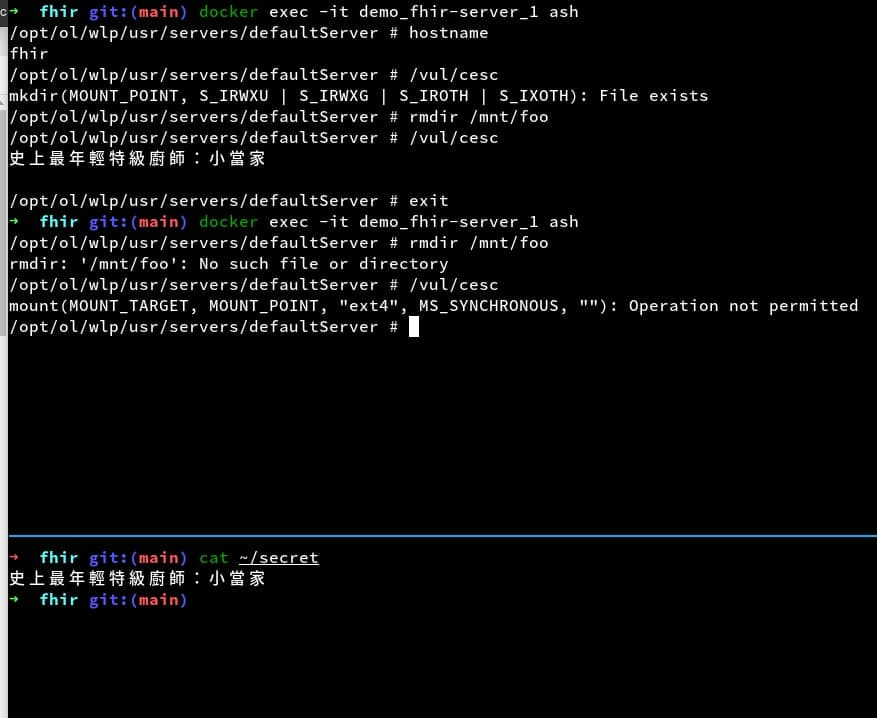
\includegraphics[width=\textwidth]{photo_2021-09-17_15-41-37.jpg}
  \end{frame}

  \begin{frame}{The container escape malware}
    \centering
    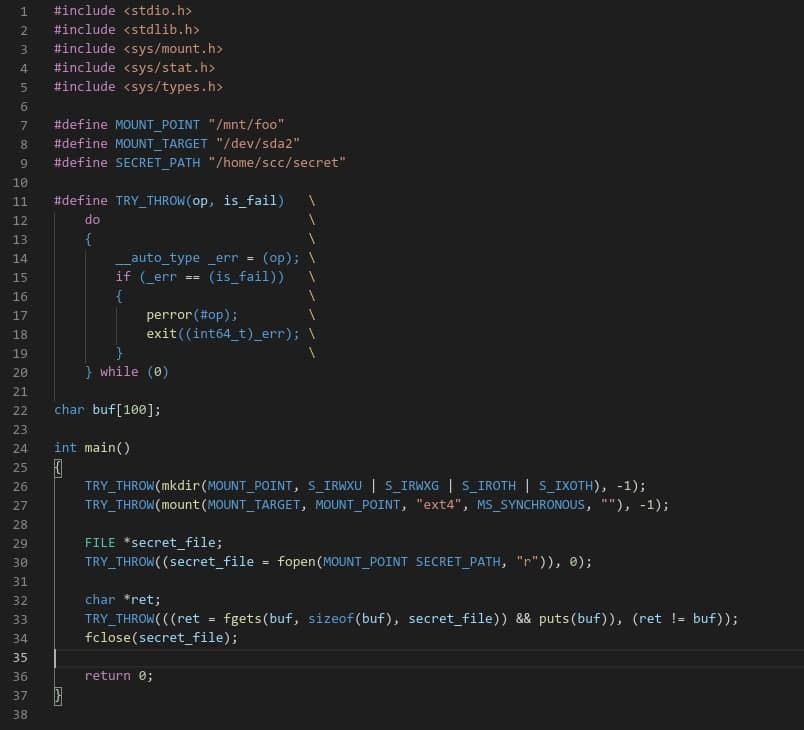
\includegraphics[height=.95\textheight]{photo_2021-09-17_06-09-47.jpg}
  \end{frame}

  \section{Performance benchmark?}

  \begin{frame}{Significant}
    \begin{multicols*}{2}
      \begin{itemize}
        \item Port my image/software to the other "container" engine or virtual machines.
        \item Benchmark: The {\color{red} cost} of defensing same vulnerability:
              \begin{itemize}
                \item My solution in docker.
                \item Using the gVisor.
              \end{itemize}
      \end{itemize}
      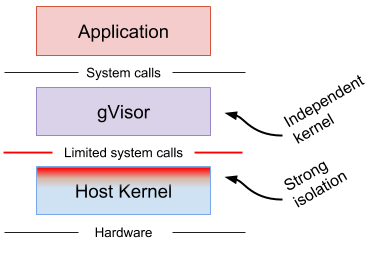
\includegraphics[width=.45\textwidth]{gvisor.png}
    \end{multicols*}
  \end{frame}

  \begin{frame}{Wait, what is gVisor?}
    gVisor is an application kernel, written in Go, that implements a substantial portion of the Linux system call interface. It provides an additional layer of isolation between running applications and the host operating system.
    \\
    gVisor’s approach is similar to User Mode Linux (UML),\\
    although UML virtualizes hardware internally and thus provides a fixed resource footprint.
  \end{frame}

  \begin{frame}{Arch and Ubuntu}
    \centering
    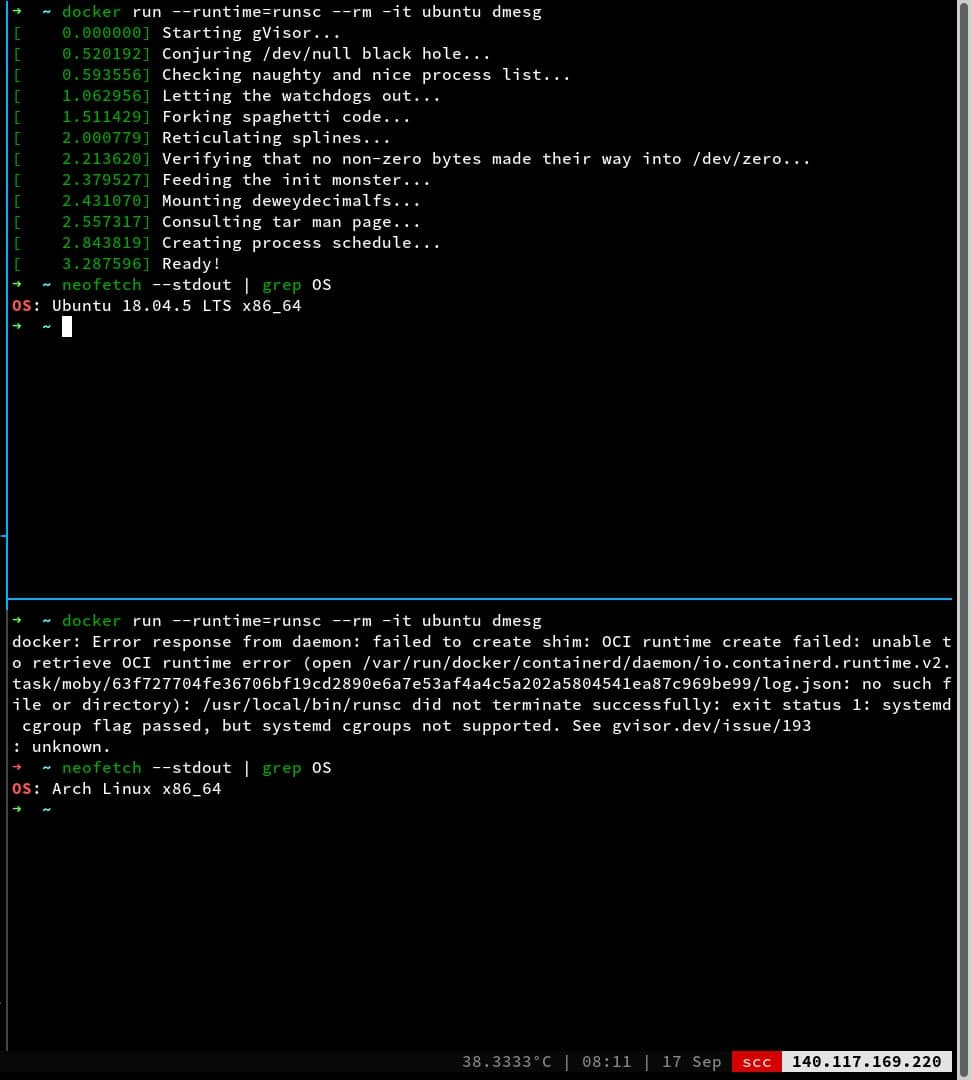
\includegraphics[height=.95\textheight]{photo_2021-09-17_15-59-52.jpg}
  \end{frame}

  \begin{frame}
    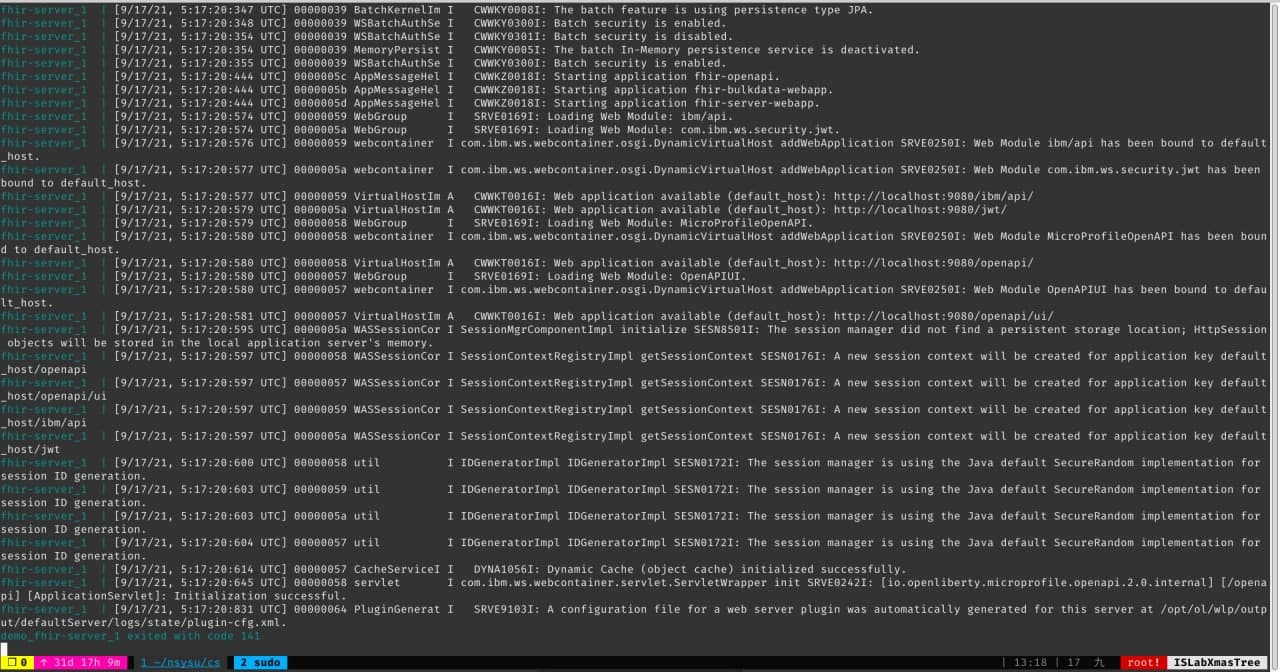
\includegraphics[width=\textwidth]{photo_2021-09-17_16-01-14.jpg}
  \end{frame}

  \begin{frame}
    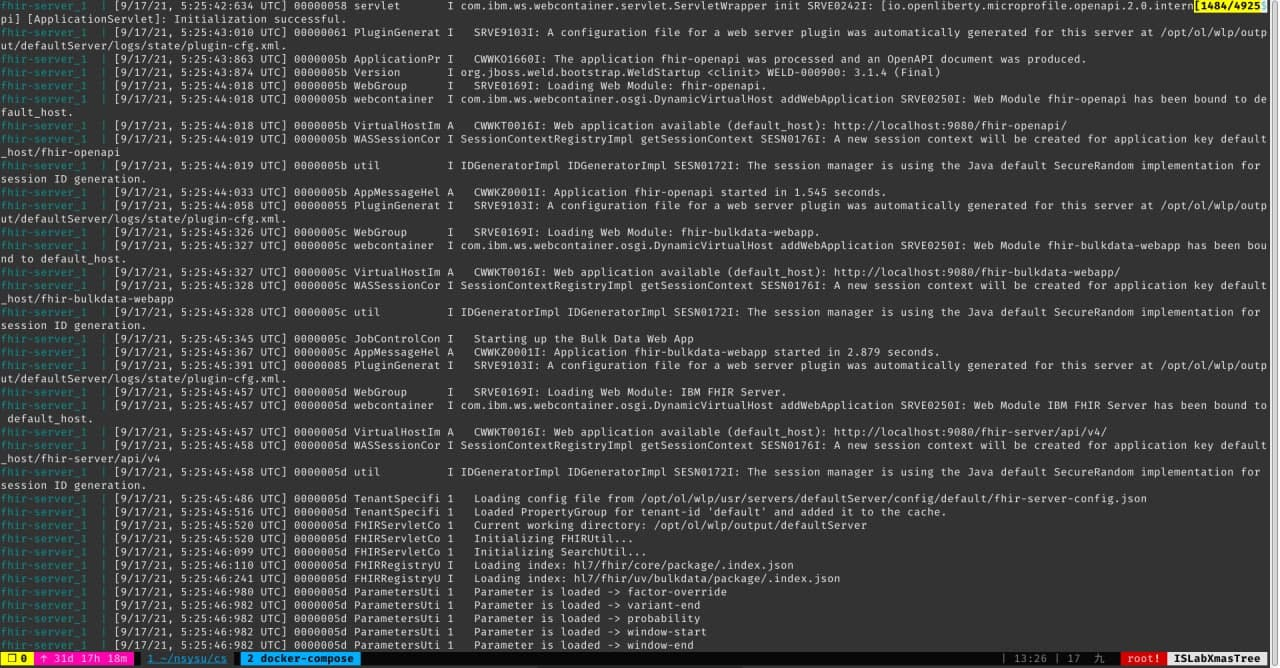
\includegraphics[width=\textwidth]{photo_2021-09-17_16-16-15.jpg}
  \end{frame}


\end{CJK*}
\end{document}